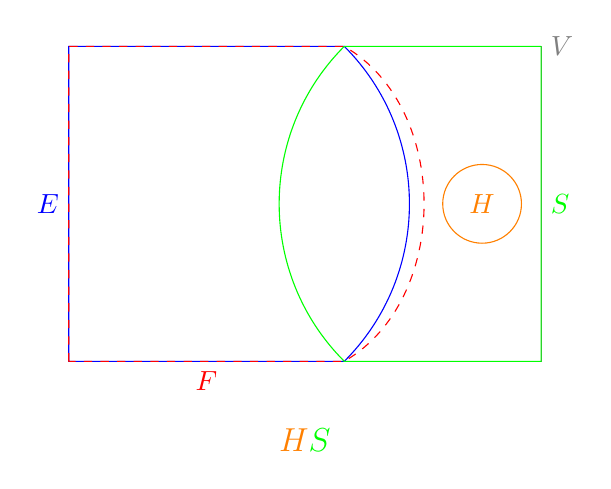
\begin{tikzpicture}
\draw[color=gray] (0,0) rectangle (6,4) node[right] {$V$};
\draw[color=blue] (0,0) -- (0,4) node[left,midway] {$E$} -- (3.5,4) to[out=-45, in=45] (3.5,0) -- (0,0);
\draw[color=red,dashed] (0,0) -- (0,4) -- (3.5,4) to[out=-30, in=30] (3.5,0) -- (0,0) node[below,midway] {$F$};
\draw[color=green] (6,4) -- (3.5,4) to[out=180+45, in=180-45] (3.5,0) -- (6,0) -- (6,4) node[right,midway] {$S$};
\draw[color=orange] (5.25,2) circle(0.5) node {$H$};
\node at (3,-1) {\large $\textcolor{orange}{H} \klgl \textcolor{green}{S}$};
\end{tikzpicture}
